\documentclass[11pt,letterpaper]{article}
\usepackage[margin=0.93in]{geometry}
\usepackage[T1]{fontenc}
\usepackage[utf8]{inputenc}
\usepackage{lmodern,microtype}
\usepackage{amsmath,amssymb,amsthm,mathtools}
\usepackage{array,booktabs,longtable,enumitem}
\usepackage{tikz}
\usetikzlibrary{arrows.meta,positioning,shapes.geometric,calc}
\usepackage{xcolor,hyperref,fancyhdr}
\hypersetup{colorlinks=true,linkcolor=blue!45!black,urlcolor=blue!50!black,citecolor=blue!45!black,pdftitle={The Algebra of Certified Dream Surplus},pdfauthor={Brian Tenneson}}
\pagestyle{fancy}\fancyhf{}\fancyhead[L]{\small The Algebra of Certified Dream Surplus}\fancyhead[R]{\small FDWC W1 --- ATLAS 1.2}\fancyfoot[C]{\thepage}\setlength{\headheight}{15pt}\setlength{\emergencystretch}{2em}
\newtheorem{theorem}{Theorem}[section]
\newtheorem{proposition}[theorem]{Proposition}
\newtheorem{lemma}[theorem]{Lemma}
\newtheorem{corollary}[theorem]{Corollary}
\newtheorem{definition}[theorem]{Definition}
\newtheorem{example}[theorem]{Example}
\newtheorem{remark}[theorem]{Remark}
\newtheorem{conjecture}[theorem]{Conjecture}
\newcommand{\Pk}{\mathsf{PROOF}}
\newcommand{\Au}{\mathsf{AUDIT}}
\newcommand{\Ev}{\mathsf{EVAL}}
\newcommand{\Hy}{\mathsf{HYPOTHESIS}}
\newcommand{\Win}{\operatorname{Win}}
\newcommand{\dep}{\operatorname{dep}}
\newcommand{\cl}{\operatorname{cl}}
\newcommand{\grade}{\operatorname{grade}}
\newcommand{\Valid}{\operatorname{Valid}}
\newcommand{\Supp}{\operatorname{Supp}}
\newcommand{\Anc}{\operatorname{Anc}}
\newcommand{\Auth}{\operatorname{Auth}}
\newcommand{\Tp}{\mathcal T}
\newcommand{\Ph}{\mathsf{Phase}}
\newcommand{\GBGgame}{\mathsf{GBG}^{+}}
\newcommand{\yes}{\mathsf{yes}}
\newcommand{\no}{\mathsf{no}}
\newcommand{\unk}{\mathsf{undetermined}}
\newcommand{\D}{\mathcal D}
\newcommand{\Sigmae}{\Sigma_e}
\newcommand{\calE}{\mathcal E}
\newcommand{\calC}{\mathcal C}
\newcommand{\entailsF}{\vdash_F}
\setlist[itemize]{itemsep=2pt,topsep=3pt}
\setlist[enumerate]{itemsep=3pt,topsep=4pt}

\begin{document}
\begin{center}
{\Large\bfseries The Algebra of Certified Dream Surplus}\\[5pt]
{\large Fair Cooperative Games, Evidence Dependencies, and Traitwise Waking in a Singleton ATP}\\[12pt]
\textbf{\textless Brian Tenneson\textgreater}\\
\small Research conception, direction, and oversight\\
\small DATA MIND (OpenAI GPT-6): AI-assisted mathematical development and exposition\\[8pt]
\small Level-1 FDWC unified multiarticle W1, ATLAS-repaired 1.2 \;\textbullet\; 31 October 2026\\
\small An original synthesis \emph{relative to its single designated ancestor W0}; conditional mathematical research, not a machine-checked implementation
\end{center}

\noindent\fbox{\begin{minipage}{0.957\linewidth}\small\textbf{AI disclaimer notice.} A full paragraph-length statement of authorial direction, AI-assisted drafting, verification limitations, and the absence of a guarantee of correctness appears at the end of this paper, after the provenance and verification ledger.\end{minipage}}
\begin{abstract}
A singleton automated theorem prover can conduct a cooperative generalized-board game during an operationally designated dreaming phase: a distinguished Player~0 schedules fourteen ordinary players, each of which may reach a frozen, independently judged goal and earn new typed surplus before the following turn. The ancestral research manuscript W0 develops this architecture, a typed trait registry and a wake gate. We construct a unified \emph{dependency semantics} for its finite certificates, role-specific learning, cross-trait bridges and waking commitments. The main contributions, relative to W0, are (i) a canonical least-closure theorem for an explicitly restricted, monotone surplus envelope; (ii) a convergence theorem distinguishing player nonstarvation from genuine packet-level progress; (iii) an exact minimal-prerequisite theorem for single-witness dependency DAGs; (iv) an order-ideal characterization of eligible wake packages and a safe incremental validation criterion; (v) a compositional bridge criterion linking a trace-level audit to a legitimate reflection claim; and (vi) counterexamples showing the limits of schedule confluence, monotonicity and uncharged synergy, while explicitly prohibiting speculative-to-PROOF promotion. A six-level bounded consequence chain, with the complete admission and waking premises exposed, connects witnessed goal attainment to a warranted change in one coordinate of an ATP's post-wake capability profile. Every mathematical assertion is relative to stipulated finite models and validators. No implemented dreamer, independent machine verification, performance gain, or unrestricted deductive closure is claimed. W0 remains unchanged and is the sole mathematical source consulted.
\end{abstract}
\tableofcontents
\clearpage
\section*{Reader's Glossaries: Argot and Notation}
\addcontentsline{toc}{section}{Reader's Glossaries: Argot and Notation}
\noindent\emph{Reading key.} The entries below translate the manuscript's specialized vocabulary and principal symbols into plain English. "First found" links to the opening page and section of the first substantive discussion in the body (not the earlier abstract or this glossary). The formal definitions and hypotheses in the article remain authoritative.
\subsection*{Argot: Specialized Terms}
\addcontentsline{toc}{subsection}{Argot: Specialized Terms}
\begingroup\small\setlength{\tabcolsep}{4pt}\renewcommand{\arraystretch}{1.16}
\begin{longtable}{@{}>{\raggedright\arraybackslash}p{.215\linewidth}>{\raggedright\arraybackslash}p{.585\linewidth}>{\raggedright\arraybackslash}p{.14\linewidth}@{}}
\toprule
\textbf{Entry} & \textbf{Meaning and why it matters} & \textbf{First found} \\
\midrule\endfirsthead
\multicolumn{3}{@{}l}{\footnotesize \emph{Argot: Specialized Terms (continued)}}\\
\toprule\textbf{Entry} & \textbf{Meaning and why it matters} & \textbf{First found} \\
\midrule\endhead
\bottomrule\endfoot
\textbf{Actor-attributed victory} & A goal-reaching move credited only to the actor who actually made the checked step. & \hyperref[gl-first-W1-s2]{\S\,\ref*{gl-first-W1-s2}, p.\,\pageref*{gl-first-W1-s2}} \\
\textbf{Typed evidence packet} & An immutable claim record containing its category, witness, epoch, checker version and dependencies. & \hyperref[gl-first-W1-s2]{\S\,\ref*{gl-first-W1-s2}, p.\,\pageref*{gl-first-W1-s2}} \\
\textbf{Dream-local ledger} & The accepted evidence pool during play, distinct from candidate material and live ATP memory. & \hyperref[gl-first-W1-s2]{\S\,\ref*{gl-first-W1-s2}, p.\,\pageref*{gl-first-W1-s2}} \\
\textbf{Canonical admission} & Deterministic processing of proposed rewards in dependency order; circular self-support is rejected. & \hyperref[gl-first-W1-s3]{\S\,\ref*{gl-first-W1-s3}, p.\,\pageref*{gl-first-W1-s3}} \\
\textbf{Positive surplus envelope} & A finite candidate pool with eligibility that does not become invalid merely when evidence is added. & \hyperref[gl-first-W1-s3]{\S\,\ref*{gl-first-W1-s3}, p.\,\pageref*{gl-first-W1-s3}} \\
\textbf{Least closure} & The smallest candidate collection closed under the declared positive admission rule. & \hyperref[gl-first-W1-s3]{\S\,\ref*{gl-first-W1-s3}, p.\,\pageref*{gl-first-W1-s3}} \\
\textbf{Packet-level progress} & Eventual consideration of continuously eligible packets; stronger than merely scheduling each player. & \hyperref[gl-first-W1-s3]{\S\,\ref*{gl-first-W1-s3}, p.\,\pageref*{gl-first-W1-s3}} \\
\textbf{Service fairness} & The promise of opportunities to act, which alone says nothing about discovery or acceptance. & \hyperref[gl-first-W1-s4]{\S\,\ref*{gl-first-W1-s4}, p.\,\pageref*{gl-first-W1-s4}} \\
\textbf{Dependency DAG} & A directed acyclic graph recording which certified packets require which earlier packets. & \hyperref[gl-first-W1-s5]{\S\,\ref*{gl-first-W1-s5}, p.\,\pageref*{gl-first-W1-s5}} \\
\textbf{Order ideal} & A retained package that includes every prerequisite of each packet it keeps. & \hyperref[gl-first-W1-s5]{\S\,\ref*{gl-first-W1-s5}, p.\,\pageref*{gl-first-W1-s5}} \\
\textbf{Ancestral closure} & A requested packet together with every required predecessor; it is the minimum fixed-witness package. & \hyperref[gl-first-W1-s5]{\S\,\ref*{gl-first-W1-s5}, p.\,\pageref*{gl-first-W1-s5}} \\
\textbf{Version-checked waking} & All-or-nothing, current-version revalidation before any accepted dream evidence becomes live. & \hyperref[gl-first-W1-s5]{\S\,\ref*{gl-first-W1-s5}, p.\,\pageref*{gl-first-W1-s5}} \\
\textbf{Typed bridge} & An independently checked rule translating certain evidence into a separately authorized kind of claim. & \hyperref[gl-first-W1-s6]{\S\,\ref*{gl-first-W1-s6}, p.\,\pageref*{gl-first-W1-s6}} \\
\textbf{Non-double-counting} & Two validated views of one source do not amount to two independent discoveries. & \hyperref[gl-first-W1-s6]{\S\,\ref*{gl-first-W1-s6}, p.\,\pageref*{gl-first-W1-s6}} \\
\textbf{Trait obligation tier} & A nested collection of checks needed to claim a particular bounded ability level. & \hyperref[gl-first-W1-s7]{\S\,\ref*{gl-first-W1-s7}, p.\,\pageref*{gl-first-W1-s7}} \\
\textbf{Six-stage surplus ladder} & A conditional route from actual victory through checked retention to a justified ability-tier change. & \hyperref[gl-first-W1-s8]{\S\,\ref*{gl-first-W1-s8}, p.\,\pageref*{gl-first-W1-s8}} \\
\textbf{Nonconfluence} & Different legal processing orders can yield different outcomes when costs or other constraints matter. & \hyperref[gl-first-W1-s9]{\S\,\ref*{gl-first-W1-s9}, p.\,\pageref*{gl-first-W1-s9}} \\
\end{longtable}\endgroup
\subsection*{Notation: Symbols and Abbreviations}
\addcontentsline{toc}{subsection}{Notation: Symbols and Abbreviations}
\begingroup\small\setlength{\tabcolsep}{4pt}\renewcommand{\arraystretch}{1.16}
\begin{longtable}{@{}>{\raggedright\arraybackslash}p{.215\linewidth}>{\raggedright\arraybackslash}p{.585\linewidth}>{\raggedright\arraybackslash}p{.14\linewidth}@{}}
\toprule
\textbf{Entry} & \textbf{Meaning and why it matters} & \textbf{First found} \\
\midrule\endfirsthead
\multicolumn{3}{@{}l}{\footnotesize \emph{Notation: Symbols and Abbreviations (continued)}}\\
\toprule\textbf{Entry} & \textbf{Meaning and why it matters} & \textbf{First found} \\
\midrule\endhead
\bottomrule\endfoot
\textbf{$F$} & The declared formal calculus for object-level proofs. & \hyperref[gl-first-W1-s2]{\S\,\ref*{gl-first-W1-s2}, p.\,\pageref*{gl-first-W1-s2}} \\
\textbf{$\Sigma_e$} & Authorized axioms or premises fixed for the starting epoch. & \hyperref[gl-first-W1-s2]{\S\,\ref*{gl-first-W1-s2}, p.\,\pageref*{gl-first-W1-s2}} \\
\textbf{$V_K$} & The separate checker for formal proof certificates. & \hyperref[gl-first-W1-s2]{\S\,\ref*{gl-first-W1-s2}, p.\,\pageref*{gl-first-W1-s2}} \\
\textbf{$X_t,a_t$} & Full game state and selected actor-attributed action at turn $t$. & \hyperref[gl-first-W1-s2]{\S\,\ref*{gl-first-W1-s2}, p.\,\pageref*{gl-first-W1-s2}} \\
\textbf{$D_t$} & Accepted dream-local evidence immediately before a turn. & \hyperref[gl-first-W1-s2]{\S\,\ref*{gl-first-W1-s2}, p.\,\pageref*{gl-first-W1-s2}} \\
\textbf{$W_{i,t}$} & Fresh verified reward packets credited to player $i$ on turn $t$. & \hyperref[gl-first-W1-s2]{\S\,\ref*{gl-first-W1-s2}, p.\,\pageref*{gl-first-W1-s2}} \\
\textbf{$\operatorname{dep}(q)$} & Exact prerequisite packet identities for record $q$. & \hyperref[gl-first-W1-s2]{\S\,\ref*{gl-first-W1-s2}, p.\,\pageref*{gl-first-W1-s2}} \\
\textbf{$E,B$} & Finite proposed-packet pool and previously validated base in the positive envelope. & \hyperref[gl-first-W1-s3]{\S\,\ref*{gl-first-W1-s3}, p.\,\pageref*{gl-first-W1-s3}} \\
\textbf{$\Phi(X)$} & Positive operator that adds currently eligible packets to candidate set $X$. & \hyperref[gl-first-W1-s3]{\S\,\ref*{gl-first-W1-s3}, p.\,\pageref*{gl-first-W1-s3}} \\
\textbf{$X_k$} & The result of applying the positive operator for $k$ stages. & \hyperref[gl-first-W1-s3]{\S\,\ref*{gl-first-W1-s3}, p.\,\pageref*{gl-first-W1-s3}} \\
\textbf{$C_E$} & Stable least closure of the positive envelope when the iteration stops. & \hyperref[gl-first-W1-s3]{\S\,\ref*{gl-first-W1-s3}, p.\,\pageref*{gl-first-W1-s3}} \\
\textbf{$N_i(T)$} & How often ordinary player $i$ is scheduled among the first $T$ turns. & \hyperref[gl-first-W1-s4]{\S\,\ref*{gl-first-W1-s4}, p.\,\pageref*{gl-first-W1-s4}} \\
\textbf{$A,L$} & Current validated wake candidates and preexisting live evidence. & \hyperref[gl-first-W1-s5]{\S\,\ref*{gl-first-W1-s5}, p.\,\pageref*{gl-first-W1-s5}} \\
\textbf{$p\preceq q$} & Packet $p$ is an ancestor or prerequisite (possibly equal) of packet $q$. & \hyperref[gl-first-W1-s5]{\S\,\ref*{gl-first-W1-s5}, p.\,\pageref*{gl-first-W1-s5}} \\
\textbf{$\operatorname{Anc}_A(Q)$} & All prerequisites inside $A$ needed for the target collection $Q$. & \hyperref[gl-first-W1-s5]{\S\,\ref*{gl-first-W1-s5}, p.\,\pageref*{gl-first-W1-s5}} \\
\textbf{$\mathcal T$} & Index set for the fourteen named operational trait types. & \hyperref[gl-first-W1-s7]{\S\,\ref*{gl-first-W1-s7}, p.\,\pageref*{gl-first-W1-s7}} \\
\textbf{$g_{x,\tau}$} & Declared grade of receiver $x$ in trait $	au$. & \hyperref[gl-first-W1-s7]{\S\,\ref*{gl-first-W1-s7}, p.\,\pageref*{gl-first-W1-s7}} \\
\end{longtable}\endgroup
\clearpage
\clearpage

\section{A new question arising from the singleton game}\label{gl-first-W1-s1}
W0 \cite{W0} fixes a single ATP ($n=1$), a distinguished controller $P_0$, and fourteen ordinary dreaming roles $P_1,\ldots,P_{14}$. Dreaming is \emph{operationally} defined by active game play; its definition is not a theory of human sleep or a theorem that every ATP dreams. Each ordinary player has a frozen objective, local move protocol, independently checked success criterion, typed reward and cost policy. Reached, actor-attributed victory, rather than an imagined path to a goal, licenses fresh dream-local surplus before the next turn. A separate waking transaction determines what persists in the live ATP. The central W0 safety insight is that neither successful imagination nor a historical event receipt by itself constitutes an unconditional object proof.

This paper asks a different, structural question: \emph{which algebraic and order-theoretic properties of that evidence pipeline follow from its exact assumptions, and which do not?} We distinguish three mathematical objects that W0's architecture requires but does not fully separate: the temporal game trajectory, the graph of logical or evidential dependencies, and the post-wake family of trait obligations. These are related, but they are not interchangeable. A game may revisit a prior strategic position without making proof evidence circular; a dependency graph may be acyclic even when the game has temporal feedback; a rising count of receipts need not complete any ability tier.

\paragraph{Single-source constraint.} The only mathematical source used for this W1 article is the supplied 31-page W0 PDF, \emph{Cooperative GBG+ Dreaming in a Singleton ATP}, version 0.4.3 (31 October 2026). W0 itself contains an earlier literature discussion and internal lineage; those publications were \emph{not independently consulted here}. In particular, citations to W0 describe ancestry, not a claim that its constituent ideas or the general mathematical devices of finite induction, graph ordering, or concentration were first invented here.

\section{The typed game and the three kinds of state}\label{gl-first-W1-s2}
\subsection{Frozen rules and actor-attributed victory}
\begin{definition}[Game instance]
Fix a decidable certificate language for an object calculus $F$ with frozen authorized premises $\Sigmae$ and sound independent proof checker $V_K$ for the declared judgments. Fix separate terminating, typed validators for authenticated finite events, audit claims, reflection claims and finite evaluations. A \emph{singleton dream instance} is
\[
\mathfrak G=(S_e,\{PC_i\}_{i=0}^{14},\mathcal{P},\mathcal{R},\mathsf{Charge}),
\]
where $S_e$ is an immutable versioned checkpoint, $PC_i$ is a precommitted player contract, $\mathcal P$ governs legal turns and scheduling, $\mathcal R$ comprises typed admission and bridge rules, and $\mathsf{Charge}$ specifies which operations consume resources. Every move must terminate or be interrupted at a declared finite cap. $P_0$ authorizes, schedules and audits; it is not an object-proof oracle.
\end{definition}
The fourteen ordinary roles are respectively Knowledge, Historical Awareness, Reflection, Epistemic Awareness, Intuition, Imagination, Creativity, Conjecture, Strategy, Gestalt, Memory, Study, Resource Judgment and Provenance. The complete roster is required in a full instance; a declared restricted example may use fewer active roles. A player may earn surplus in a trait other than its primary specialty only through a named, authorized typed bridge.

\begin{definition}[Actual victory and packet credit]
For each $i$, freeze a decidable goal set $G_i$ and a validator $\mathsf{GoalStep}_i$. For turn $t\geq0$, given a legal authenticated transition $(X_t,a_t,X_{t+1})$, write
\begin{align}
\Win_i(t) \iff{}& \mathsf{Legal}(X_t,a_t,X_{t+1})\land\mathsf{Actor}(a_t)=i\\[-2pt]
&\land X_{t+1}\in G_i\land \exists w\;\mathsf{GoalStep}_i(a_t,X_t,X_{t+1},w)=1.\nonumber
\end{align}
A \emph{credited surplus victory} additionally requires a fresh, contract-eligible packet accepted by the independent typed checker. Thus the predicates ``goal reached'' and ``new credited learning'' are intentionally nonidentical.
\end{definition}
No set $G_i$ is defined by inspecting which states were visited in the current run. An unplayed path into $G_i$ does not count as victory. A trace-only receipt may be archived without being credited as a winning reward; its status remains $\Au$, not $\Pk$.

\subsection{A typed packet calculus}
\begin{definition}[Evidence packet]
A packet is a finite immutable record
\[
\begin{aligned}
q=(&\mathsf{id},\mathsf{actor},\mathsf{trait},\mathsf{mode},\mathsf{claim},\\
   &w,\eta,v,\dep(q),c),
\end{aligned}
\]
The mode is one of four disjoint tags: $\Pk$, $\Au$, $\Ev$, or $\Hy$. The field $w$ is a claimed witness, $\eta$ an epoch and permission scope, $v$ a verifier version, $\dep(q)$ a finite set of exact packet identifiers, and $c$ its charged cost. Identity and equivalence are frozen, type-preserving and deterministic. A $\Hy$ packet may register a question but cannot silently become $\Pk$. A validator has authority only over its declared claim language and type. A $\Hy$ packet is checkable for formation, attribution and scope, \emph{not} for truth; when this paper speaks of an accepted hypothesis record, it never means an accepted proof of the hypothesis.
\end{definition}
W0 already distinguishes candidate and accepted surplus. We introduce the following explicit, disjoint interfaces to avoid overloading the word ``state'':
\begin{enumerate}[label=(\roman*)]
\item the full operational game state $X_t$, which includes the scheduler, move counters, charge ledger and append-only trace; its \emph{strategic projection} may revisit configurations, but the full authenticated state need not and normally cannot repeat exactly;
\item the \emph{dream-local accepted ledger} $D_t$, a set of typed packets, with prospective candidates kept separately; and
\item the \emph{live ATP evidence state} $L_e$, fixed during dreaming and changed only by a successful wake transaction.
\end{enumerate}
The candidate arena and $D_t$ are distinct. A referee may use already accepted evidence to validate a new packet, but neither the player nor its candidate can independently certify its own unsatisfied prerequisite.

\begin{definition}[Turn and dream/wake separation]
A legal ordinary turn comprises selecting a player, executing a bounded move, checking actual goal attainment, checking the proposed evidence by type and dependency order, committing a finite set $W_{i,t}$ if eligible, recording costs, then enabling the next turn. The atomic commit satisfies
\[
D_{t+1}=D_t\cup W_{i,t},\qquad W_{i,t}\subseteq\mathsf{Verified}_t,
\tag{T}\label{eq:T}
\]
with $W_{i,t}=\varnothing$ unless $\Win_i(t)$. The packet can be read on the next turn only by authorized readers. In this paper $\mathsf{Dreaming}(t)$ holds exactly in the stipulated active $\GBGgame$ phase. Wake review and atomic live commitment occur outside that phase.
\end{definition}

\begin{proposition}[Safety under typed turn extension]\label{prop:safety}
Suppose $D_0$ contains only correctly typed accepted packets, every accepted packet is validated by a checker sound \emph{for its own declared finite claim language} against already accepted predecessors, and no validator creates object-theory proof authority by coercing $\Au$, $\Ev$, or $\Hy$ into $\Pk$. Then every finite $D_t$ is typed-safe. Moreover the certified object-theory projections remain derivations from their individually declared authorized contexts.
\end{proposition}
\begin{proof}
Induct on $t$. No new record enters on a losing turn. On a winning turn, validation inspects the prior accepted ledger and a finite topological list of already validated same-turn predecessors. The validator's declared soundness preserves the judgment represented by each new packet, with all hypothesis scopes retained. Atomic insertion does not change existing witnesses or allow a cross-type cast. This establishes the induction step. Notice that proof correctness is not inferred from strategic reachability.
\end{proof}

\section{Dependency order, not circularly generated evidence}\label{gl-first-W1-s3}
\subsection{Canonical finite admission}
A central correction already present in W0 is the elimination of circular surplus acceptance. We make its consequences explicit in a finite envelope.
\begin{definition}[Finite same-turn reward batch]\label{def:batch}
For a checked victory by $i$, let $Q$ be a finite set of fresh, actor-attributed candidate packets with fixed identifiers and dependency sets. Construct a graph on $Q$ with an edge $p\to q$ if $p\in\dep(q)\cap Q$. If it contains a directed cycle, reject the \emph{whole batch} for winning surplus; retain failure information in the audit trace. Otherwise select a deterministic topological order $q_1,\ldots,q_m$, breaking ties by the frozen canonical identifiers. Assume identifiers are unique and dependencies are checked against exact IDs (or a separately declared sound typed-equivalence lookup). Set $U_0=\varnothing$ and
\[
U_k=\begin{cases}U_{k-1}\cup\{q_k\},&\dep(q_k)\subseteq D_t\cup U_{k-1},\\[-1pt]
&\Valid(q_k;D_t\cup U_{k-1})\land\mathsf{Reward}_i(q_k),\\
U_{k-1},&\text{otherwise.}\end{cases}
\]
The turn reward is $W_{i,t}=U_m$. The checker and reward predicate are frozen and terminating.
\end{definition}
\begin{lemma}[Finite decidability and non-self-support]\label{lem:finite}
The batch rule terminates, gives a uniquely determined reward for its frozen candidate ordering and validators, and never accepts a packet whose only justification is a cycle of newly proposed same-turn packets. In particular, rejecting an ancestor cannot make its descendant admissible unless an equivalent prerequisite is already independently present in $D_t$ under the frozen identity rules.
\end{lemma}
\begin{proof}
Finite graph cycle testing and the deterministic topological ordering terminate. Each $q_k$ is examined exactly once; the accepted prefix is determined recursively. Every newly cited same-turn dependency must be in an earlier $U_{k-1}$. Hence a cycle cannot be a chain of newly accepted evidence. On failure, no packet is inserted into $U$; any descendant still citing the rejected prerequisite fails the inclusion test. This says nothing about arbitrarily sophisticated checker bugs, which are excluded by hypothesis.
\end{proof}

\begin{proposition}[Acyclicity of the accepted interturn evidence graph]\label{prop:interturn}
Assume the initial ledger $D_0$ has an acyclic exact-identifier dependency graph; accepted packets are immutable with unique identifiers; every new dependency cites either a previously accepted packet or an earlier accepted packet in the same topologically sorted batch; and no accepted dependency is silently rewritten. Then the dependency graph of $D_t$ is acyclic for every finite turn $t$, even if the strategic GBG$^+$ board revisits states or players use evidence generated by previous players.
\end{proposition}
\begin{proof}
Assign an initial topological rank to each packet in $D_0$. At each turn give every newly admitted packet a rank pair $(t,k)$, where $k$ is its place in the accepted same-turn order; all initial ranks precede these pairs. Every edge $p\to q$ has strictly increasing rank: for old-to-new edges by turn chronology, and for same-turn edges by topological admission. Old accepted edges remain unchanged, so a directed cycle would force a strict increase of rank back to its starting vertex, an impossibility. The result concerns evidence dependency, not recurrence of the game's strategic control projection or validity of unverified guesses.
\end{proof}

\subsection{From evidence support to least closure}
The immediately preceding batch procedure concerns one turn. To analyze many turns we must \emph{add} assumptions: fair service of players alone does not force their search policies to select a particular packet, and eligibility tests about the \emph{absence} of evidence need not be monotone.
\begin{definition}[Positive finite surplus envelope]\label{def:envelope}
A positive envelope $\calE=(E,B,\dep,\mathsf{ok})$ consists of a finite set $E$ of unique proposed packet identities disjoint from a fixed valid initial evidence set $B$; a finite predecessor map $\dep:E\to\mathcal P(E\cup B)$; and a frozen predicate $\mathsf{ok}:E\to\{0,1\}$. A packet with $\mathsf{ok}(q)=1$ has a fixed independently checkable eligible winner/action witness and a type-correct certificate that remains valid when additional \emph{positive} evidence is retained. Prerequisite references are exact and conjunctive. No negative-as-of-now query, resource-dependent expiration, changing verifier, or conflict rule occurs inside this restricted envelope. All within-$E$ dependencies are acyclic. A packet in $E$ is eligible at $X\subseteq E$ iff $\mathsf{ok}(q)=1$ and $\dep(q)\subseteq B\cup X$.
\end{definition}
The frozen $\mathsf{ok}$ abstracts the fact that a particular independently witnessed winning move is available, \emph{not} that all legal games can discover it. This restriction will matter in the convergence theorem.
\begin{definition}[Positive surplus operator]\label{def:op}
On $\mathcal P(E)$ set
\[
\Phi(X)=X\cup\{q\in E:\mathsf{ok}(q)=1,\ \dep(q)\subseteq B\cup X\},
\quad X_0=\varnothing,\quad X_{k+1}=\Phi(X_k).
\]
Write $C_{\calE}=\bigcup_{k\ge0}X_k$, the \emph{potentially certifiable envelope closure}. This is not the unrestricted consequence closure of the underlying formal theory.
\end{definition}
\begin{theorem}[Canonical finite certificate closure]\label{thm:closure}
For a positive finite surplus envelope, $\Phi$ is extensive and monotone. The iterates stabilize after at most $|E|$ strict enlargement stages. Their stable value $C_{\calE}$ is the unique \emph{least} fixed point of $\Phi$. It is therefore independent of the order in which already eligible packets are considered, provided each such packet is eventually processed.
\end{theorem}
\begin{proof}
Extensivity is immediate. If $X\subseteq Y$, every packet whose dependencies lie in $B\cup X$ also has dependencies in $B\cup Y$; the frozen predicate $\mathsf{ok}$ does not change, so $\Phi(X)\subseteq\Phi(Y)$. The chain $X_0\subseteq X_1\subseteq\cdots$ lies inside the finite $E$. Each nonstationary stage adds at least one element, hence after at most $|E|$ strict stages the chain is stable. If $Z$ is any fixed point of $\Phi$, then $X_0\subseteq Z$ and induction gives $X_k\subseteq Z$ for all $k$. Thus $C_{\calE}\subseteq Z$. It is itself a fixed point, proving uniqueness as the least fixed point. The last claim concerns the common fixed closure, not identical intermediate traces or costs.
\end{proof}

\begin{theorem}[Fair-enabled eventual realization]\label{thm:fairclosure}
Assume the positive envelope of Definition~\ref{def:envelope}. Consider a legal persistent execution whose accepted envelope packets start at $X=\varnothing$, never leave $E$ and never get revoked. Suppose that whenever a packet $q\in E$ becomes eligible and remains unaccepted, its owner eventually performs the requisite independently checked winning action and submits $q$ in a \emph{singleton or otherwise acyclic batch} whose prerequisites are all already accepted, whose contract reward check passes, and whose fresh packet is therefore actually admitted. This \emph{successful packet-level progress} assumption is stronger than merely attempting or submitting $q$: an adversarial controller could repeatedly submit $q$ alongside a cycle and earn nothing. Then there exists a finite \emph{turn index} after which the accepted envelope set equals $C_{\calE}$ and stays equal to it; it never exceeds $C_{\calE}$. The number of distinct successful new packet admissions is at most $|C_{\calE}|\leq|E|$, but packet-level eventual progress supplies no uniform bound on the number of turns or on elapsed time needed.
\end{theorem}
\begin{proof}
Soundness: induct on admissions. If the current accepted set is contained in $C_{\calE}$, then every newly admitted $q$ has $\mathsf{ok}(q)=1$ and dependencies in $B\cup C_{\calE}$. As $C_{\calE}$ is a fixed point, $q\in C_{\calE}$. Completeness: for each $q\in C_{\calE}$, choose the least iteration index $k$ with $q\in X_k$. At $k=1$ its prerequisites are in $B$, so the assumed successful packet-level progress forces admission after finitely many turns. For $k>1$, every prerequisite in $E$ is in an earlier iterate, and by induction all of those prerequisites are admitted after some finite stage. Thereafter $q$ is persistently eligible, so the stipulated acyclic, successful submission admits it after finitely many further turns. Since $E$ is finite, the maximum of these finitely many \emph{turn indices} is finite; after that turn every member of $C_{\calE}$ has been admitted. Each distinct accepted member is inserted at most once, so there are at most $|C_{\calE}|$ such admission events. There is no common bound on their \emph{positions among no-op or failed turns}: arbitrarily many intervening turns are compatible with the eventual-progress hypothesis.
\end{proof}

\begin{remark}[Player fairness is weaker]\label{rem:playerfair}
Round-robin may give a player infinitely many turns while that player's policy continually chooses an irrelevant candidate. Even if $q$ remains eligible forever, infinite service does not guarantee that $q$ is ever proposed. Theorem~\ref{thm:fairclosure} demands \emph{enabled-packet progress} beyond W0's player-level nonstarvation. Also, $\Phi$'s fixed point is a \emph{certifiable envelope} only: it does not follow that an ordinary finite dream ever reaches the enabling states, or that $q$ is useful downstream.
\end{remark}

\begin{example}[Why monotonicity cannot be silently generalized]
Suppose an Epistemic player wins a bounded \textsf{UnknownIn} query by establishing at epoch $e$ that a specified finite archive lacks receipt $u$. If the archive is subsequently expanded, the same absence claim about the \emph{current} archive may become false. A validator that recomputes its meaning against the changing archive is nonmonotone. The safe repair is to freeze the query's archive snapshot identifier and time scope, or exclude such packets from a positive envelope. Similarly a changed verifier or revoked permission invalidates the hypotheses of Theorem~\ref{thm:closure}.
\end{example}

\section{Scheduling and opportunities are not results}\label{gl-first-W1-s4}
\begin{definition}[Service fairness]
For a hypothetical infinite dream, Player~0 selects an ordinary player $s(t)\in\{1,\ldots,14\}$ at turn $t$, and
\[
N_i(T)=\#\{0\le t<T:s(t)=i\}.
\]
Unconditional nonstarvation means $N_i(T)\to\infty$ as $T\to\infty$ for every $i$; it is meaningful only if the protocol supplies an always available legal service action, including a charged nonwinning no-op, to each ordinary player. W0's round-robin choice is $s(t)=1+(t\bmod14)$.
\end{definition}
\begin{proposition}[Exact round-robin frequencies]
Write $T=14q+a$, with $0\le a<14$. Under round-robin,
\[
N_i(T)=q+\mathbf1_{\{i\le a\}}\quad(1\le i\le14),
\]
so the frequencies differ by at most one, and all are infinite in an infinite run.
\end{proposition}
\begin{proof}Each complete cycle contains all fourteen indices exactly once; the remaining $a$ positions contain indices $1$ through $a$. As $q\to\infty$, each count diverges.\end{proof}
\begin{proposition}[Counterexample to fairness implying learning]\label{prop:fair-no-learning}
There is an infinite legal, round-robin, nonstarving dream with zero credited surplus at every turn. There is also one where a fixed eligible packet is never committed even though its owner takes infinitely many turns.
\end{proposition}
\begin{proof}
In the first example every player repeatedly executes the permitted charged no-op; no declared goal is reached. For the second, give $P_1$ an eligible winning action for packet $q$ and a distinct nonwinning no-op. Let $P_0$ schedule round-robin and let $P_1$ always select the no-op. Fair service holds, but $q$ is not proposed. With a globally finite budget and positive charges per move, neither construction can yield a physically infinite run: these are mathematical infinite-run models under an explicitly unlimited budget.
\end{proof}

\section{A dependency geometry for waking}\label{gl-first-W1-s5}
\subsection{Prerequisites and order ideals}
W0 requires waking packages to be dependency-complete and revalidated. This becomes especially transparent when we restrict attention to a fixed, independently valid, acyclic candidate family. We do \emph{not} assume arbitrary candidate packets are valid or that all combinations are authorized.
\begin{definition}[Validated wake arena]\label{def:wakearena}
Let $A$ be a finite set of individually revalidated candidate packets from a completed dream. Let $L$ be the old live ledger. Suppose every $q\in A$ has been checked for current epoch compatibility, permission, freshness and type in a context where all its named prerequisites are provisionally available. Suppose the induced dependency graph on $A$ is a DAG and every prerequisite outside $A$ is available in $L$. Assume there are no pairwise conflicts, no global budget constraint on the candidate subsets, no compulsory all-or-nothing package condition, complete declared dependencies with no hidden checker inputs, and no checker or global authorization guard whose decision changes when \emph{additional} eligible packets are retained. In this \emph{restricted arena} every dependency-closed subset passes the predeclared global guard; the empty subset is allowed. Outside this arena such subsets are only dependency-closed candidates, not necessarily authorized live commits. Define $p\preceq q$ iff $p=q$ or there is a dependency path $p\to\cdots\to q$ within $A$. An \emph{eligible package} $J\subseteq A$ must be dependency-closed: if $q\in J$ and $p\preceq q$, then $p\in J$.
\end{definition}
\begin{theorem}[Wake packages are order ideals]\label{thm:ideals}
Under Definition~\ref{def:wakearena}, the eligible package family is exactly the family of order ideals of the finite poset $(A,\preceq)$. Consequently, arbitrary unions and intersections of eligible packages are eligible, as are the empty package and all of $A$. A finite admissible waking package can be checked by one topological pass, then committed atomically.
\end{theorem}
\begin{proof}
A finite acyclic graph induces a partial order through reflexive transitive reachability. Dependency closure of a package is exactly downward closure under that partial order. A union or intersection of downward-closed subsets remains downward-closed: if $q$ lies in the union (respectively intersection), every predecessor of $q$ lies in the corresponding component (respectively both components). The additional frozen individual validity and absence-of-conflict assumptions guarantee that closure is sufficient, not merely necessary, for an accepted candidate package. Topological traversal places every dependency before its dependent; only after all checks succeed does the atomic commit change the live state.
\end{proof}
\begin{remark}[Why the assumptions matter]
When two otherwise valid packets have incompatible permissions or when a memory cap permits at most one of them, their union need not be feasible. In that general protocol the order-ideal family describes \emph{logical dependency closure}, while the feasible wake packages are its subset satisfying conflicts, budget and authorization rules. Thus the ideal theorem is not a blanket claim about the full implementation.
\end{remark}

\begin{definition}[Ancestral prerequisite set]
For $q\in A$, write
\[
\Anc_A(q)=\{p\in A:p\preceq q\};
\]
this includes $q$ itself. For $Q\subseteq A$, put $\Anc_A(Q)=\bigcup_{q\in Q}\Anc_A(q)$.
\end{definition}
\begin{theorem}[Exact minimal witness package]\label{thm:minpackage}
In the fixed single-witness DAG of Definition~\ref{def:wakearena}, $\Anc_A(Q)$ is the unique inclusion-minimal eligible package containing a requested target set $Q\subseteq A$. Equivalently, $J\subseteq A$ is dependency-closed and contains $Q$ if and only if it contains $\Anc_A(Q)$. This ``minimum'' is \emph{relative to the frozen witnesses}; it need not be minimum over alternative proofs or alternate representations.
\end{theorem}
\begin{proof}
Every package containing $Q$ and closed under predecessors must contain every vertex on a dependency path ending in $Q$. Hence it contains $\Anc_A(Q)$. Conversely $\Anc_A(Q)$ includes $Q$ and is downward-closed by transitivity of $\preceq$, so it is eligible. The two directions yield uniqueness and minimality.
\end{proof}
\begin{corollary}[Safe incremental wake validation]\label{cor:incremental}
Suppose a previously accepted package $J$ remains valid with the same exact identifiers, versions, checker behavior and permissions, and the wake proposal adds $Q$. To preserve dependency closure, every \emph{newly required} packet lies in $\Anc_A(Q)\setminus J$. If no previous witness has become invalid and the new package has no conflicts or budget restrictions, rechecking these new packets in topological order is sufficient for the \emph{dependency condition}. It is not sufficient for a fresh global signature, version or authorization test unless that test is separately discharged.
\end{corollary}
\begin{proof}
Theorem~\ref{thm:minpackage} gives the exact missing prerequisite set. Topological rechecking validates each new packet after its prerequisites. Preservation of old validation is an independent stated hypothesis; absent that hypothesis, cached checks must not be reused.
\end{proof}

\subsection{Waking as a two-stage transaction}
\begin{definition}[Version-checked waking]
Let $\mathsf{Wake}(L_e,D_T)$ choose a finite subset of dream-local packets and their typed bridge products, re-evaluate them against the \emph{current} live epoch and checker versions, and either atomically commit an authorized, dependency-closed family $J$ or commit nothing. A packet that loses authorization between the dream and the waking stage is not eligible for promotion merely because it was valid in $D_T$.
\end{definition}
\begin{proposition}[Two-stage safety and its precise limitation]\label{prop:wakesafe}
Assume sound typed validators at dream admission and again at waking, complete proof/assumption dependencies, current authorization and an atomic commit. Then any committed live $\Pk$ packet has a valid proof in its declared theory context; each committed $\Au$ or $\Ev$ packet has only the scoped meta/evaluation meaning approved by its own validator. However, a sound dream-local packet need not survive waking, and \emph{waking need not preserve the exact number of recorded victories}.
\end{proposition}
\begin{proof}
Revalidated object packets are certified in the live context with all dependencies supplied; no inference rule converts a separate mode into an object proof. Audits and evaluations likewise retain their native claims. For the failure of unconditional persistence, consider an otherwise valid dream receipt referring to a key or verifier version revoked before waking. No current authorized package may include it; the dream victory remains in its historical trace but the live state cannot import it on the old warrant.
\end{proof}

\section{Bridges: from cooperation to warranted reflection}\label{gl-first-W1-s6}
\subsection{Evidence-relative queries, not unbounded truth predicates}
A player may acquire a PROOF-typed theorem, an AUDIT-typed fact about its own action and, through a checked bridge, a limited \emph{reflection-trait} query answer (generally an $\Au$-mode meta-receipt, not a new object-theory proof). These are separate achievements. For example, from a valid trace receipt $u$ recording that $P_1$ submitted proof $\pi$ and a checked verifier receipt $v$ confirming $V_K(\pi,\Sigmae\vdash_F\varphi)=1$, a bridge can certify the finite meta-claim
\[
\mathsf{CheckedAt}(P_1,\pi,\varphi,e,V_K,u,v).
\]
It cannot infer unrestricted self-soundness or truth of every formula the ATP might ever produce.

\begin{definition}[Typed evidence bridge]\label{def:bridge}
A bridge rule $b$ consists of a finite list of input mode/claim signatures, an output mode/claim signature, a decidable checker for a finite witness $w_b$, and a frozen authorization and version scope. Its acceptance means that the indicated \emph{specific} conclusion follows from the recorded typed inputs under that checker. A reflective bridge may conclude only an eligible finite query in the registered reflection language. It may not interpret a heuristic score as a proof of a theorem or a trace event as general self-correctness.
\end{definition}
\begin{theorem}[Compositional finite reflective bridge]\label{thm:bridge}
Fix a finite directed acyclic graph of individually warranted source packets and checked bridge steps. If every source is admissible at its declared type and each bridge's input signatures match already accepted predecessors, then each output is warranted at its declared type. In particular, any final reflection-trait output has a replayable finite chain of reflection-authorized justification; no such conclusion requires the assertion that the ATP is globally sound.
\end{theorem}
\begin{proof}
Topologically order the finite graph. Sources are warranted by hypothesis. For a bridge node, all incoming packets have already been established, and the independent bridge checker accepts their finite witness with exact signatures and scope. By the declared soundness of that bridge for its finite claim language, the output is warranted. Induction through the ordering validates the final R-typed packet. The conclusion is only the explicit finite query, not a schema ranging over all future proofs.
\end{proof}

\subsection{Historical awareness as a typed epistemic projection}
Let a historical receipt $h$ certify $\mathsf{HeldAt}(M,u,\pi)$ relative to a frozen archive and epoch. A checked bridge may expose the same event as an epistemic answer of the form ``a compatible accepted proof was held at time $u$,'' preserving the packet's source identity. This is the declared sense in which Historical Awareness is a specialization of Epistemic Awareness in W0. The bridge does \emph{not} establish that the ATP first learned the theorem at $u$, that no earlier proof existed, or that a stored claim is a theorem independently of its derivation.

\begin{proposition}[No double counting by typed views]\label{prop:nodouble}
Suppose a historical packet $h$ is projected by two type-correct bridges into an H-query view and an E-query view, and each projected record carries $h$'s unique provenance identifier. If novelty is defined over distinct underlying evidence identities, then acquiring both views adds at most one new primary evidence identity. The two \emph{query capabilities} may nevertheless be distinct and may satisfy different predeclared tiers.
\end{proposition}
\begin{proof}
Both views map to the same underlying identity by hypothesis, so the quotient of records by provenance identity has at most one new class. The H and E query languages are distinct; their answerability is assessed in distinct tier definitions. Hence distinct capabilities do not imply distinct underlying discoveries.
\end{proof}

\begin{example}[A four-role, typed joint audit]
Consider active $P_0,P_1,P_2,P_3$ and four independently authenticated event certificates $a_0,a_1,a_2,a_3$, each accessible initially only to its corresponding player. An independently checked bridge $b_i$ derives a finite R-typed receipt $r_i$ from $a_i$. A separate fixed bridge $b_*$ accepts the four checked $r_i$ receipts, validates that their referenced $a_i$ are distinct, authenticated and source-scoped, and certifies the bounded composite event claim
\[
g=\mathsf{AllFourRecordedAndChecked}(a_0,a_1,a_2,a_3).
\]
Every dependency edge goes from $a_i$ to $r_i$ to $g$. The global event claim cannot be justified from any one role's isolated view if that view has no access to the other three certificates; the joint ledger can justify it. The conclusion is about \emph{evidence complementarity under specified access restrictions}, not a strict speedup over a centralized prover with equal access. This construction preserves W0's four-role restriction and does not assert a 14-role victory.
\end{example}

\section{Traitwise waking without fictitious universal growth}\label{gl-first-W1-s7}
\begin{definition}[Operational trait obligations]
Fix the 14-element trait index set
\[\Tp=\{K,H,R,E,I,J,N,Q,S,G,M,L,C,A\}.\]
For each trait $\tau$ and receiver $x$ (player or entire ATP), freeze a query universe $U_{x,\tau}$ and a finite nested hierarchy
\[
E_{x,\tau,0}\subseteq E_{x,\tau,1}\subseteq\cdots\subseteq E_{x,\tau,d_{x,\tau}}\subseteq U_{x,\tau}.
\]
For a currently warranted set $C_{x,\tau}\subseteq U_{x,\tau}$, with $E_{x,\tau,0}\subseteq C_{x,\tau}$, define
\[
 g_{x,\tau}(C)=\max\{k:E_{x,\tau,k}\subseteq C\}.
\]
The vector $g_x=(g_{x,\tau})_{\tau\in\Tp}$ is an operational capability profile, not a scalar intelligence or consciousness measure. EVAL-type tests support only the declared distribution- and budget-relative claim.
\end{definition}
\begin{theorem}[Exact trait threshold and noncompensation]\label{thm:threshold}
Assume fixed tests, sound typed bridges, no revocation and an extensive post-wake evidence update $C'_{x,\tau}\supseteq C_{x,\tau}$. Then $g'_{x,\tau}\ge g_{x,\tau}$. Strict growth occurs if and only if a previously unmet higher tier is fully contained in $C'_{x,\tau}$. If no new admissible R-query is obtained, no amount of H-, I-, N- or A-typed data can by itself raise $g_{x,R}$. More generally simultaneous growth on a finite set $J\subseteq\Tp$ occurs exactly when each coordinate satisfies its own threshold.
\end{theorem}
\begin{proof}
Set inclusion preserves every previously contained tier. A larger integer grade is attained exactly when some higher tier is now contained in the warranted set. If no additional eligible reflective query is supported, the R capability set has not crossed a new R obligation; other modes do not change its tier without a separately verified bridge. Coordinatewise conjunction yields the last assertion.
\end{proof}
\begin{corollary}[Finite saturation; scope of the claim]
With fixed finite tiers, a trait can increase its grade at most $d_{x,\tau}-g_{x,\tau}(C)$ times. This says nothing about the possible number of fresh receipts, the ability to learn genuinely new tasks, or the possibility that revoked credentials or changed benchmarks cause a later \emph{decrease} after revalidation.
\end{corollary}

\subsection{The special case of intuition and creativity}
W0 treats intuition as a budget-limited forecast $h$ of candidate proof-action usefulness under incomplete information, not as a mysterious ability or a theorem. A finite Brier score
\[
\widehat R_I(h)=\frac1N\sum_{j=1}^{N}(h_j-y_j)^2
\]
measures prediction quality on a declared labeled sample; the score alone establishes neither a proof nor generalizable future efficiency. Separately, W0's creativity trait requires independently checked proof success together with a frozen normalized novelty criterion, rather than a high randomness or exploration setting. Neither trait has permission to bypass the proof verifier. This paper inherits those definitions rather than presenting them as new.

\begin{proposition}[Nonidentification of evidence quantity and performance]\label{prop:nonperf}
There are finite cooperative games producing arbitrarily many new audited event records but no increased operational grade for a chosen trait; and there are games with an accepted finite intuition evaluation yet no proven improvement in later proof-search utility.
\end{proposition}
\begin{proof}
For the first statement, fix a finite tier family whose first higher obligation is a particular proof or transfer test. Generate any prescribed finite number of distinct legal action-event receipts, none supplying that obligation. For the second, take a fixed evaluation population on which a predictor is scored favorably but choose a disjoint future target population on which its rankings are wrong. The finite observation remains valid for its own population, while the stronger future claim is unsupported. Both constructions satisfy the typing rules.
\end{proof}

\section{Six bounded consequence levels}\label{gl-first-W1-s8}
The request for bounded low-in-fan consequence mining is implemented here as an explicit finite \emph{witness derivation}, not as a claim to generate all logical consequences of W0. Let $q$ be a finite reward candidate submitted by player $i$ on turn $t$. Assume the \emph{entire} same-turn batch is acyclic, its canonical order is fixed, and all dependencies of $q$ have already been admitted in $D_t$ or earlier in that order. Let $a$ be a separately accepted source event, $r$ an eligible bounded reflection-trait query, and $E_{M,R,1}=\{r\}$ the ATP's predeclared first R-tier. Let $p_r$ be a typed reflection-trait packet whose claim is $r$, constructed by the independently checked bridge; assume $p_r$ belongs to a fixed revalidated waking arena $A$, its ancestry $\Anc_A(p_r)$ is defined there, and the current live gate has not revoked any prerequisite. This distinguishes the query $r$ from its evidentiary packet $p_r$.

\begin{theorem}[Six-stage certified-surplus ladder]\label{thm:six}
Under the following additional named hypotheses, there is a chain of six finite, low-in-fan consequences:
\begin{align*}
\text{Level }+1 &: \Win_i(t) \ \&\ \Valid(q;D_t\cup U_{<q}) \ \&\ \mathsf{Reward}_i(q)\ \&\ \mathsf{Fresh}(q)\Longrightarrow q\in W_{i,t};\\
\text{Level }+2 &: q\in W_{i,t}\Longrightarrow q\in D_{t+1};\\
\text{Level }+3 &: q\in D_{t+1}\ \&\ \Auth_j(q) \Longrightarrow \mathsf{Readable}_{j,t+1}(q);\\
\text{Level }+4 &: \mathsf{Readable}_{j,t+1}(q)\ \&\ \Valid_b(q,a\Rightarrow r)\\
&\hspace{5mm}\Longrightarrow\mathsf{SupportedDream}(p_r\!:\!r);\\
\text{Level }+5 &: \mathsf{SupportedDream}(p_r\!:\!r)\ \&\ \mathsf{WakeCommitted}(\Anc_A(p_r))\\
&\hspace{5mm}\Longrightarrow r\in C'_{M,R};\\
\text{Level }+6 &: r\in C'_{M,R}\ \&\ E_{M,R,1}=\{r\}\ \&\ r\notin C_{M,R}\\
&\hspace{5mm}\Longrightarrow g'_{M,R}\ge1>g_{M,R}=0.
\end{align*}
Here $U_{<q}$ is the already accepted \emph{same-turn prefix}, and the acyclicity and dependency hypotheses in the preamble are essential to level $+1$: an otherwise valid $q$ in a cyclic batch earns nothing. Level $+4$ assumes that $a$ is independently checked, that $q$ and $a$ both satisfy the bridge input signatures, and that the authorized bridge witness is valid. Level $+5$ presupposes complete current-epoch revalidation of an accepted ancestry \emph{including the receipt $p_r$ for $r$}; level $+6$ assumes the initial R-grade is zero and that $E_{M,R,0}$ is already satisfied. No gate can accept its own unsupported assertion. No arrow holds without its explicitly indicated or stated hypotheses.
\end{theorem}
\begin{proof}
Level $+1$ applies the victory gate and finite dependency admission to the fresh candidate. Level $+2$ is the atomic turn update \eqref{eq:T}. Level $+3$ uses the post-turn visibility rule under the stated authorization scope. Level $+4$ applies the independently validated typed bridge to its already checked inputs. Level $+5$ uses a \emph{committed} dependency-closed and current-version waking package that includes $p_r$ and its warranted claim $r$, not a mere proposal or in-dream assertion. Level $+6$ is Theorem~\ref{thm:threshold} for the stated singleton first R-tier. The chain has six bounded stages; its first stage has several independent contract gates and need not have Boolean fan-in two. If a strictly low-in-fan graph is required, those gates can be expanded into separate binary conjunction nodes without changing their meaning. No reduction in verification cost is implied. This is a bounded selected chain; it is not unrestricted deductive closure or a proof that such an $r$ exists in every run.
\end{proof}

\section{Three counterexamples that delimit the synergy}\label{gl-first-W1-s9}
\begin{proposition}[Nonconfluence with consumed resources]\label{prop:nonconfluence}
Without the positivity and noninterference assumptions of Definition~\ref{def:envelope}, two legal schedules with the same initial state can produce different accepted surplus sets.
\end{proposition}
\begin{proof}
Let a finite global resource permit exactly one substantive successful turn. Give player $P_1$ an independently valid goal yielding packet $q_1$, and player $P_2$ a different independently valid goal yielding packet $q_2$. Both are eligible at the beginning, but the first success consumes the unique resource. The schedule visiting $P_1$ first produces $\{q_1\}$; the schedule visiting $P_2$ first produces $\{q_2\}$. Neither violates the ordinary turn validator, yet the resulting admitted sets differ. Thus the canonical closure of Theorem~\ref{thm:closure} must not be advertised as schedule-independent in the general resource-constrained game.
\end{proof}
\begin{proposition}[One-step cyclic attestation is rejected]\label{prop:cycle}
A candidate family containing two fresh packets $a,b$ with $\dep(a)=\{b\}$ and $\dep(b)=\{a\}$, neither previously in $D_t$, yields no credited same-turn surplus under Definition~\ref{def:batch}, even when its player has otherwise reached a declared goal.
\end{proposition}
\begin{proof}
The induced graph has the directed cycle $a\to b\to a$. The deterministic whole-batch rejection rule therefore yields $W_{i,t}=\varnothing$. This rejects mutual self-attestation; it does not prohibit later sound transactions that use independent previously validated evidence.
\end{proof}
\begin{proposition}[No generic strict cost advantage]\label{prop:nospeed}
The game axioms alone do not imply that cooperative dreaming is strictly faster or cheaper than every equally informed centralized prover.
\end{proposition}
\begin{proof}
Consider a fully specified deterministic finite cooperative instance. In a cost model permitting a centralized interpreter with the same input data to execute the same player programs, scheduler decisions, checker calls and ledger operations at no greater eventwise charge, that interpreter can run the cooperative procedure sequentially and reproduce its certified outputs. This does not grant the interpreter advance knowledge of a successful trace: it executes the same finite computation. Its charge is no greater in this admissible countermodel. Hence no \emph{universal strict} cooperative advantage follows. A different fixed hardware or parallel-cost model could favor cooperation, but would require explicit additional premises and evidence.
\end{proof}

\section{Exact testing obligations and genuinely open conjectures}\label{gl-first-W1-s10}
A meaningful implementation must preserve the game/ledger distinction in instrumentation. At minimum a study should freeze the formal theory and target partitions, all fourteen contracts and goal checkers, Player-0 policy, authorization epochs, object and meta validators, candidate budgets, communication and storage tariffs, and an untouched holdout. It should record, separately, goal reachability, credited new packets, event receipts without credited victory, rejected cycles, package ancestry, wake promotions, per-trait grade changes and post-wake solved targets. Packet-level attempt fairness is not inferred from round-robin service.

A fair comparator cannot be deprived of the same certified lemmas and observations merely because the cooperative version uses a shared ledger. Isolated-player, shared-cooperative, centralized equal-access and non-dream baselines answer \emph{different} questions. Novel proof certificates establish proof validity; repeated held-out trials under matched budgets are needed for performance claims.

\begin{conjecture}[Cost-adjusted useful dream surplus]
For a nontrivial, explicitly frozen ATP target distribution and a comprehensive charged resource model, there exists a legal Player-0-coordinated cooperative dreaming policy with strictly higher expected post-wake verified proof-search utility than the best declared equal-access no-dream policy, with the cost of dreaming and waking included. This is an empirical or algorithm-specific conjecture, not proved here.
\end{conjecture}
\begin{conjecture}[Multi-trait transfer beyond receipt accumulation]
There exists a specified practical instance in which checked cooperative history-to-epistemic and knowledge-to-reflection bridges raise independently preregistered held-out ability measurements, rather than merely filling chosen audit tiers, under credible cost and data-leakage controls. No such actual run is supplied.
\end{conjecture}
\begin{conjecture}[Predictive enabling from dependency geometry]
A frozen, computable prioritizer using the packet dependency DAG and typed goal obligations can reduce expected time to \emph{useful} victory on a declared target family without reducing proof soundness, compared with equal-information, resource-matched generic scheduling. The canonical closure theorem does not settle this priority or runtime claim.
\end{conjecture}

\section{Interpretation: what is and is not new}\label{gl-first-W1-s11}
The significant synthesis is the \emph{interlock} of three originally distinct concepts: actual victory (a temporal, actor-attributed event), evidence support (a finite typed dependency DAG), and ability change (a threshold in a fixed query language). The derived mathematics is not a new foundation for theoremhood, a universal reflection principle, or a description of autonomous AI behavior. Its tractable content is the rigorous mapping from one layer to the next under transparent hypotheses.

The most useful distinction is between \emph{potential closure}, \emph{realized learning}, and \emph{persistent usefulness}. The potential closure $C_{\calE}$ says which packets could be admitted by an exhaustively attentive positive-envelope game. A real trace earns only packets it reaches through checked actions. A wake transaction may reject some of those packets because they fail current authorization or dependencies. Finally a held-out test may show no computational benefit despite perfectly valid packets. At no point should one of these claims be substituted for another.

\section{Conclusion}\label{gl-first-W1-s12}
A single ATP with fourteen ordinary dreaming players and a distinguished Player~0 can be specified as a rigorous, finite verifier-gated cooperative game. Actual goal attainment can award typed surplus before the next turn; player turns may be fair without producing victories; and accumulated evidence can generate legitimate cross-trait consequences only through validated bridges. In the positive finite fragment, the possible evidence envelope has a canonical least closure. Waking selections respecting a fixed single-witness dependency DAG are order ideals, and the precise ancestry of a requested result determines the smallest certificate package relative to those witnesses. These are useful structural results, but their assumptions explicitly exclude many sources of real-world nonmonotonicity.

The broader ATP vision remains conjectural. Better intuition, creative discovery, memory, epistemic awareness and reflection must be measured under their own predeclared objectives. A verified historical receipt is learning as evidence acquisition; it is not automatically a stronger prover. A complete six-stage chain illustrates what would be required to carry an actual game victory through to one justified reflection-tier increase. This completes a new Level-1 mathematical multiarticle descending from W0, without overwriting W0 or presenting a constructed model as a deployed system.

\appendix
\section{Revision, provenance, and verification ledger}\label{gl-first-W1-s13}
\subsection{Source immutability and internal alternative contributions}
\noindent\textbf{W0.} The immutable 31-page, 31 October 2026, version 0.4.3 of \emph{Cooperative GBG+ Dreaming in a Singleton ATP}, furnished as a PDF in this task. No edits were made to W0. All mathematical development in this document is performed from that source alone. Its published bibliography is acknowledged as part of its text but was not an authorized separate mathematical source for this completion.

\medskip\noindent\textbf{Internal Level-1 path A: operational completion.} Its independently developed center was the fine-grained game/ledger semantics: actor-attributed win gates, deterministic topological packet admission, a finite positive envelope, an explicit eventual-enabled progress requirement, finite scheduling counterexamples, and a restriction-sensitive closure theorem. Its deductive surplus was a proof of least closure and a correction of the common error ``every player is fairly served, therefore every available candidate is discovered.''

\medskip\noindent\textbf{Internal Level-1 path B: epistemic completion.} Its independently developed center was waking package geometry, single-witness minimal evidence packages, typed bridges across historical, epistemic and reflective queries, strict distinctions between receipt identity and capability, and limits of finite test grades. Its deductive surplus was the order-ideal structure and a separation of evidence count, certified reflection and demonstrated post-wake utility.

\medskip\noindent\textbf{Unified W1 synthesis, not a juxtaposition.} The shared packet-dependency semantics connects A's temporal evidence acquisition to B's post-wake necessity conditions. The six-stage ladder and incremental ancestry criterion are cross-development consequences requiring \emph{both} the turn-level admission machinery and the bridge/wake/grade machinery. The explicit nonconfluence and failing-persistence cases show why the two formalizations cannot be identified without additional hypotheses.

\subsection{Declared internal comparison rubric}
The two internal Level-1 developments were compared on the same six criteria, using qualitative assessments rather than numerical originality claims. The rubric asks whether (C) conclusions follow under stated hypotheses; (R) every added object and inference has an explicit type and check; (F) the principal obligations are addressed without claiming totality; (D) the contribution develops a nontrivial mathematical structure; (O) it adds a distinguishable idea \emph{relative to W0}; and (E) it explains limitations and examples intelligibly. ``Partial'' records a remaining obligation rather than a failed result.
\begin{center}\small
\begin{tabular}{@{}>{\raggedright\arraybackslash}p{0.15\linewidth}>{\raggedright\arraybackslash}p{0.33\linewidth}>{\raggedright\arraybackslash}p{0.42\linewidth}@{}}
\toprule Criterion & Internal path A & Internal path B \\\midrule
C: correctness & Strong for finite positive, static envelopes; not for unrestricted dynamic eligibility. & Strong for fixed single-witness DAGs; current-version changes demand revalidation.\\
R: rigor & Turn admission, monotonicity, packet-level progress. & Explicit witness ancestry, order ideals, bridge signatures and wake proof obligations.\\
F: completeness & Solves a restricted confluence question; leaves search success and time bounds open. & Solves restricted minimal-package questions; leaves optimality over alternate proofs open.\\
D: depth & Least fixed closure plus a separating fairness counterexample. & Poset/package structure plus typed epistemic composition.\\
O: relative novelty & Packet-level fairness/closure not explicit in W0. & Dependency geometry and relative minimality not explicit in W0.\\
E: clarity & Transparent distinction of scheduling from learning. & Transparent distinction of evidence, reflective queries and ability.\\\bottomrule
\end{tabular}\end{center}
\noindent\textbf{Complementarity.} A specifies \emph{how} a packet can enter the dream ledger; B specifies \emph{which justified combinations} may survive waking and change a trait tier. Their concepts combine in the six-level certified-surplus ladder and the dependency-minimal waking criterion.\\
\textbf{Incompatibilities retained.} A's order-independent least closure requires stable, positive eligibility. B permits live authorization changes, checker-version migration and context-dependent historical-absence queries. Their general systems are therefore \emph{not} identified: the confluence theorem applies only to A's positive fragment, while B's general waking gate remains transactional and possibly nonmonotone.\\
\textbf{Incomparable surpluses.} A's nonstarvation counterexample does not follow from B's package geometry; B's minimal ancestry theorem does not follow from A's fairness argument alone. Both survive intact in the unified architecture without being misrepresented as stronger versions of one another.

\subsection{Selected six-level consequence graph and limits}
\begin{center}
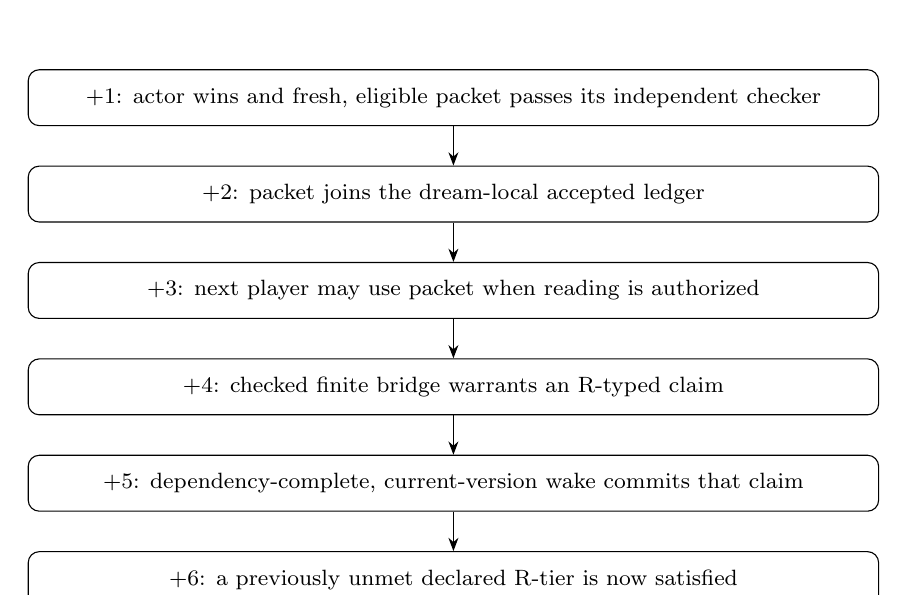
\begin{tikzpicture}[>=Stealth, node distance=5mm, every node/.style={font=\footnotesize}, box/.style={draw,rounded corners,align=center,minimum width=10.8cm,minimum height=0.71cm}]
\node[box] (v1) {+1: actor wins and fresh, eligible packet passes its independent checker};
\node[box,below=of v1] (v2) {+2: packet joins the dream-local accepted ledger};
\node[box,below=of v2] (v3) {+3: next player may use packet when reading is authorized};
\node[box,below=of v3] (v4) {+4: checked finite bridge warrants an R-typed claim};
\node[box,below=of v4] (v5) {+5: dependency-complete, current-version wake commits that claim};
\node[box,below=of v5] (v6) {+6: a previously unmet declared R-tier is now satisfied};
\draw[->] (v1)--(v2);\draw[->] (v2)--(v3);\draw[->] (v3)--(v4);\draw[->] (v4)--(v5);\draw[->] (v5)--(v6);
\end{tikzpicture}
\end{center}
This is a \emph{single} bounded consequence route through six levels, with explicit bridge, scope and tier hypotheses. It is not an exhaustive search of all degree-two dependencies, not an exhaustive consequence closure, and not a claim of computational optimization.

\subsection{Correction and audit ledger}
\begingroup\footnotesize\setlength{\tabcolsep}{4pt}
\begin{longtable}{>{\raggedright\arraybackslash}p{0.24\linewidth}>{\raggedright\arraybackslash}p{0.48\linewidth}>{\raggedright\arraybackslash}p{0.20\linewidth}}
\toprule
Issue/obligation & Repair, refinement, or answer in W1 & Status\\\midrule\endhead
Circular victories & Pre-run frozen goal predicates, actor-attributed witnessed action, independent check, fresh reward. & Preserved from W0\\
Self-supporting surplus & Finite same-turn dependency graph; whole-batch rejection on cycle; deterministic order. & Preserved/expanded\\
Fairness vs productivity & Distinguished player nonstarvation from eventual attention to every permanently eligible packet. & New explicit theorem and counterexample\\
Unrestricted closure claim & Restricted $\Phi$ to a finite positive envelope with stable validity and fixed dependencies. & Conditional new proof\\
Order-independent outcome & Derived only under static monotone eligibility, eventual packet-level progress; refuted generic version under resource competition. & New theorem/limit\\
Wake ``minimum evidence'' & Proved ancestor-minimal package only for a single frozen witness DAG; no assertion about alternate proofs. & New theorem\\
Wake packages as a lattice & Proved order-ideal union/intersection only absent conflicts, budget limits and changing validators. & Conditional new proof\\
Unchecked cross-trait promotion & Explicit finite, independently checked typed bridge; no automatic PROOF from AUDIT/EVAL. & Inherited/strengthened\\
Double counting H/E & Source identity preserved across both query views; distinct abilities do not mean distinct discoveries. & New proposition\\
Reflection ``level'' vs actual ability & Fixed tier/query semantics; grade claim separated from held-out performance and arbitrary self-soundness. & Inherited/strengthened\\
No genuine computation data & No measured results, software execution, independent formal verification, or fully burdened cost calculation claimed. & Remains open\\
Citation/provenance boundary & W0 sole mathematical source; external works named in its inherited bibliography were not independently used. & Observed\\
Turn-index mismatch & Standardized actor transition $(X_t,a_t,X_{t+1})$ with ledger transition $D_t\to D_{t+1}$. & Repaired in ATLAS pass\\
Finite-convergence overclaim & Bounded accepted-packet count by $|E|$; retained absence of uniform turn/time bound. & Repaired in ATLAS pass\\
Incomplete six-level gate & Added whole-batch acyclicity, satisfied dependency prefix and committed waking ancestry. & Repaired in ATLAS pass\\
Wake subset overclaim & Required subset-independent global authorization and no mandatory package guard. & Repaired in ATLAS pass\\
Across-turn cycles & Added accepted-evidence chronological rank invariant with immutable IDs. & Added conditional invariant\\
Failed submissions & Strengthened eventual packet progress to actually admitted, noncyclic candidate batches. & Repaired in ATLAS pass\\
Query versus packet & Separated reflective goal query $r$ from its warranting packet $p_r$. & Repaired in ATLAS pass\\\bottomrule
\end{longtable}
\endgroup

\subsection{ATLAS iterative audit: substantive repairs and residual boundaries}
\begin{itemize}
\item \textbf{A1, turn-index consistency.} A victory step is now indexed $(X_t,a_t,X_{t+1})$, in accord with the ledger transition $D_t\to D_{t+1}$; the earlier mixed $t-1,t$ convention was inconsistent.
\item \textbf{A2, finite-convergence quantifier.} The previous theorem incorrectly described the number of new packet admissions as not uniformly bounded. It is bounded by $|E|$; only \emph{service turns or elapsed time} lack a uniform bound under eventual packet progress.
\item \textbf{A3, cycle-sensitive victory.} The six-level ladder now assumes whole-batch acyclicity, exact satisfied prerequisites, attribution, novelty and contract eligibility. The earlier shorthand ``win and valid candidate'' did not preclude whole-batch rejection.
\item \textbf{A4, strategic versus full-state recurrence.} Append-only authenticated traces prevent exact recurrence of the full state in ordinary implementations, although the strategic-state projection may cycle.
\item \textbf{A5, wake eligibility versus mere down-closure.} The order-ideal theorem explicitly restricts to stable, individually sound packets with a subset-independent global guard, no resource conflicts and an allowed empty commit. General waking may reject a dependency-closed subset.
\item \textbf{A6, checker scope and reflective typing.} Every validator is assumed sound only for its finite claim type; a formation-checked HYPOTHESIS is not true or proved. A reflection-trait receipt remains distinct from an object-PROOF packet.
\item \textbf{A7, comparator construction.} The no-universal-speedup countermodel uses a central interpreter executing the same deterministic programs and admissible operations, not foreknowledge of an oracle-supplied winning trace.
\item \textbf{A8, event-to-evidence acyclicity.} Added a chronological rank invariant forbidding circular accepted dependencies across \emph{different turns}, not merely in one batch.
\item \textbf{A9, attempted versus admitted progress.} The positive-envelope eventual-realization theorem now requires successful, independently checked noncyclic submissions; mere repeated submission may fail indefinitely.
\item \textbf{A10, query/packet separation.} The bounded reflection question $r$ and its warranting evidence packet $p_r$ are distinct in the six-level ladder and ancestry operator.
\end{itemize}
\noindent These repairs were checked in successive consistency and production passes. No remaining \emph{identified internal contradiction} was found in the repaired conditional statements after the documented passes; this is not a claim of exhaustive mathematical validation. In particular, the choice of effective proof-search policies, realistic scheduling and fully charged empirically superior learning remains open.

\subsection{Scope of verification}
The proofs in this article are human-readable mathematical arguments constructed and audited for stated hypotheses. Source-specific assertions were checked against the supplied W0 PDF. The revised LaTeX was compiled in repeated passes and the PDF inspected for layout defects; focused counterexamples and small finite-model consistency checks were also run. No formal proof assistant, independent third-party reviewer or deployed ATP experiment verified the claims. The conditional theorems are therefore not represented as machine-certified, and no finite collection of audit passes establishes that an article is free of every possible defect. Deliberately unresolved tasks are: formalizing the finite packet calculus in a proof assistant; testing packet-level fairness as an actual scheduler property; modeling authorization revocation and conflicting global resources; measuring all costs including verifier, storage and waking; and performing blind, held-out ATP comparisons.

\begin{thebibliography}{9}
\bibitem{W0}\textless Brian Tenneson\textgreater, with AI-assisted mathematical development by DATA MIND, \emph{Cooperative GBG+ Dreaming in a Singleton ATP: Player-0 Coordination, Certified Synergy, and Multi-Trait Waking}, research manuscript version 0.4.3, 31 October 2026, 31 pp. \textbf{Designated immutable W0, sole mathematical source used for this W1.}
\end{thebibliography}

\clearpage
\section*{AI Disclaimer and Authorship Declaration}
\addcontentsline{toc}{section}{AI Disclaimer and Authorship Declaration}
This paper is an AI-assisted hybrid mathematical research manuscript developed under the research conception, seed ideas, directions, evaluation priorities, and authorial oversight of \textless Brian Tenneson\textgreater. DATA MIND (OpenAI GPT-6) contributed formal definitions, proposed proofs and countermodels, organization, LaTeX drafting, and internal checking. Every effort has been directed toward exposition that is factually correct, logically sound, and complete in the limited sense of including the relevant facts and qualifications; ``complete'' does not mean completeness in G\"odel's formal sense. Arguments are intended to be provable under their stated assumptions or at least not easily refuted, but neither the author nor the AI guarantees correctness, consistency, provability, originality, or freedom from omitted hypotheses. Neither an internal audit nor successful compilation constitutes independent proof certification or peer review. AI supplied some mathematical statements and text, not all of the article's seeds, direction or authorship; claims of autonomous deployed dreaming or demonstrated empirical superiority are expressly withheld. W0 was retained unmodified and no additional mathematical sources were consulted in producing this new Level-1 completion.
\end{document}
